\ExamPart{Trắc nghiệm trả lời ngắn}{2}{Thí sinh trả lời từ câu 1 đến câu 4.}

\NQuestion Cho đồ thị hàm số $y=f\left(x\right)$ như hình vẽ dưới đây.
\begin{center}
    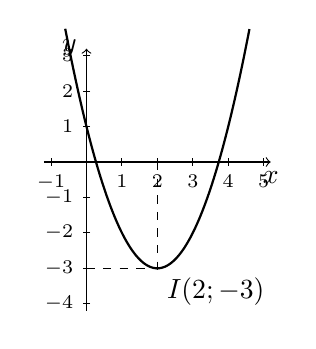
\begin{tikzpicture}[scale=0.45]
    \draw[->] (-1.2,0) -- (5.2,0) node[below] {$x$};
    \draw[->] (0,-4.2) -- (0,3.2) node[left] {$y$};

    \foreach \x in {-1,1,2,3,4,5}
        \draw (\x,0.1) -- (\x,-0.1) node[below] {\scriptsize $\x$};

    \foreach \y in {-4,-3,-2,-1,1,2,3}
        \draw (0.1,\y) -- (-0.1,\y) node[left] {\scriptsize $\y$};

    \draw[smooth, samples=200, domain=-0.6:4.6, thick]
        plot (\x, {\x*\x - 4*\x + 1});

    \fill (2,-3) circle (1.3pt);
    \draw[dashed] (2,0) -- (2,-3);
    \draw[dashed] (0,-3) -- (2,-3);
    \node[below right] at (2,-3) {$I(2;-3)$};
\end{tikzpicture}

\end{center}
Tìm giá trị nhỏ nhất của hàm số $f\left(x\right)$.
\AnswerLine{$-3$}
\SolutionBlock{Từ đồ thị, parabol mở lên và có đỉnh là $I(2;-3)$. Do đó giá trị nhỏ nhất của hàm số là $-3$.}

\NQuestion Phương trình $x^4-10x^2+9=0$ có bao nhiêu nghiệm thực?
\AnswerLine{$4$}
\SolutionBlock{Đặt $t=x^2\ (t\ge0)$. Khi đó ta được phương trình
\[
t^2-10t+9=0\Leftrightarrow (t-1)(t-9)=0.
\]
Suy ra $t=1$ hoặc $t=9$. Tương ứng, $x=\pm1$ hoặc $x=\pm3$. Vậy phương trình có $4$ nghiệm thực.}

\NQuestion Từ các chữ số $1,2,3,4,5,6$, lập được bao nhiêu số tự nhiên lẻ có $3$ chữ số đôi một khác nhau?
\AnswerLine{$60$}
\SolutionBlock{Muốn số lập được là số lẻ thì chữ số hàng đơn vị có $3$ cách chọn: $1,3,5$. Sau đó chữ số hàng trăm có $5$ cách chọn và chữ số hàng chục có $4$ cách chọn. Vậy có $3\cdot5\cdot4=60$ số.}

\NQuestion Một mảnh đất hình chữ nhật có chiều dài hơn chiều rộng $4\,\text{m}$ và diện tích bằng $96\,\text{m}^2$. Tính chu vi của mảnh đất.
\AnswerLine{$40\,\text{m}$}
\SolutionBlock{Gọi chiều rộng là $x\,(x>0)$, khi đó chiều dài là $x+4$. Theo đề bài:
\[
x(x+4)=96\Rightarrow x^2+4x-96=0\Rightarrow (x+12)(x-8)=0.
\]
Vì $x>0$ nên $x=8$. Suy ra chiều dài là $12$ m. Chu vi mảnh đất là
\[
2(8+12)=40\,\text{m}.
\]}
